\documentclass{article}
\usepackage[utf8]{inputenc}
\usepackage[portuguese]{babel}
\usepackage[a4paper]{geometry}
\usepackage{graphicx}
\usepackage{float}
\usepackage{verbatim}
\usepackage[bottom]{footmisc}
\PassOptionsToPackage{hyphens}{url}\usepackage{hyperref}
\usepackage[style=numeric]{biblatex}
\usepackage{csquotes}
\addbibresource{references.bib}

\begin{document}

\begin{titlepage}
    \center
    \begin{figure}[H]
        \centering
        
\includegraphics[width=4cm]{UM_EENG.jpg}
    \end{figure}
    \textsc{\LARGE Universidade do Minho} \\ [1.5cm]
    \textsc{\Large Mestrado Integrado em Engenharia Informática} \\ [0.5cm]
    \textsc{\large System Deployment \& Benchmarking} \\ [0.5cm]
    
    \vspace*{1cm}
    
    \rule{\linewidth}{0.5mm} \\ [0.25cm]
    {\huge \bfseries Deployment e Monitorização do GitLab}
    \rule{\linewidth}{0.5mm} \\ [0.25cm]
    
    \vspace*{1cm}

    a78821 - José Carlos Lima Martins \\
    a78587 - Ricardo Jorge Marques Peixoto \\
    a75587 - Pedro Alexandre Alves Marta \\[0.25cm]

    \today
\end{titlepage}

\begin{abstract}
O presente projeto consiste no deployment, monitorização e avaliacão da instalação distribuída da aplicação GitLab cimentando assim, os conteúdos lecionados no âmbito da unidade curricular de \textit{System Deployment and Benchmarking}, ao realizar a automatização do processo de \textit{deployment} e de \textit{benchmarking}.

A automatização do processo de instalação, configuração e benchmarking de uma aplicação foi conseguida usando o Ansible, ferramenta esta que possui muitas funcionalidades que facilitam a automatização, desde os módulos, às variàveis bem como a integração do Jinja2.

Numa primeira fase, foi realizado o deployment da aplicação sem monitorização. Como se pretende que a aplicação tenha boa escalabilidade e resiliência a falhas, a mesma é instalada numa arquitetura distribuída, onde os seus vários componentes estão dispersos por várias máquinas havendo ainda a replicação de alguns desses componentes.

Já numa segunda fase, são instaladas todas as ferramentas necessárias para a monitorização da arquitetura, usando a ELK Stack. A ELK Stack possui diversas ferramentas que variam consoante a finalidade: recolha de métricas (beats),  agregação/filtragem/tratamento de dados (Logstash), análise de dados (Elasticsearch) e ainda uma visualização final dos dados após findas as fases descritas (Kibana).

Por fim, numa terceira fase, é instalado o Apache JMeter que permite criar e executar testes sobre a arquitetura construída. Nesta fase, são realizados vários testes com o objetivo principal de identificar a capacidade máxima da aplicação, em termos de número de utilizadores e tempo de espera, no acesso à página inicial.
\end{abstract}

\newpage

\tableofcontents

\newpage

\section{Introdução}
O GitLab pode ser usado durante todo o ciclo de desenvolvimento de um projeto/aplicação, gerindo e gravando as mudanças do mesmo. Para além disso possui variadas ferramentas que ajudam no desenvolvimento e gestão de um projeto entre as quais CI (Continuous Integration) e CD (Continuous Deployment). O controlo de versões usado é o Git. Existe uma versão ``online'' (\url{https://gitlab.com}) acessível a todos (registo grátis) com os recursos disponíveis na aplicação (anualidade para ter todos os recursos, o mesmo se passa com a aplicação). Contudo a versão aplicacional permite ser ``self hosted'', ou seja, qualquer pessoa/empresa que pretenda ter o seu GitLab pode tê-lo a correr nos seus equipamentos ou onde bem pretender (por exemplo, o Google Cloud Platform), sendo que a maior parte das razões para tal escolha, envolve segurança, integração e/ou leis.
\par Portanto, tendo em conta estes aspetos será apresentado na secção \ref{Arq} qual é a arquitetura bem como quais os componentes da aplicação. De seguida, na secção \ref{Inst} é apresentada a automatização do processo de deployment bem como arquitetura usada e ferramentas usadas. A seguir, na secção \ref{Mon}, refere-se as ferramentas de monitorização usadas e as métricas usadas. Por fim, na secção \ref{Av} é feita uma avaliação ao sistema e na secção \ref{Conc} encontra-se uma breve conclusão do trabalho desenvolvido.

\section{Arquitetura e Componentes da Aplicação} \label{Arq}

\begin{figure}[H]
    \centering
    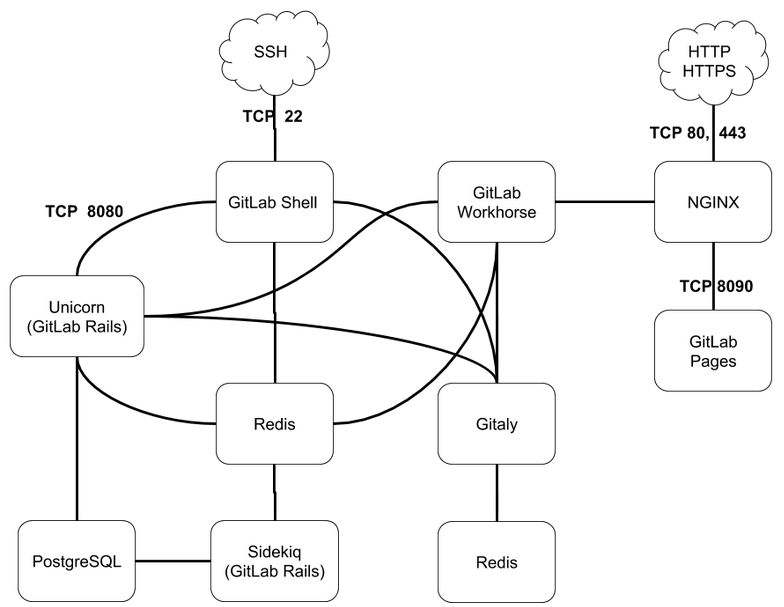
\includegraphics[width=15cm]{arch.png}
    \caption{Arquitetura do GitLab}
    \label{fig:arch}
\end{figure}

Pela figura, é possível identificar-se os vários constituintes do GitLab.~\cite{arch}

Em primeiro lugar, encontra-se um web front-end usado como proxy para o Unicorn/Workhorse sendo que este front-end tanto pode ser Nginx como Apache. Contudo, o Gitlab usa por predefinição o Nginx sendo possível configurar o GitLab de modo a usar o Apache.~\cite{apache} 

Já em relação ao Unicorn/Workhorse, são workers que servem as páginas web e a API do GitLab a utlizadores, ou seja, faz tarefas do Sidekiq.

Para além disso, o Sidekiq é também um worker mas, faz o \texit{scheduling} de filas de trabalho, e como tal, usa o Redis para obter os trabalhos, sendo estes distribuídos e são lhes atribuídos prioridades.

Como referido anteriormente, o Redis é uma base de dados não persistente para informações de trabalhos, trabalhos recebidos(a realizar, queue do Sidekiq), metadados, cache e as sessões dos utilizadores. De modo a garantir alta disponibilidade do Redis é aconselhável o uso de Sentinel's que verificam a integridade do Redis, bem como, caso o master vá abaixo, seja escolhido outro master dos slaves disponíveis (numa arquitetura master-slaves).

Em quase todas as aplicações é necessário armazenar informação de forma persistente, e o GitLab é um desses casos. Para isso, é usado o PostgreSQL (recomendável pelo GitLab) ou o MySQL de modo a guardar informações de utilizadores, permissões, issues, branches, hooks e outros metadados de forma persistente.

Já a API do GitLab resolve a autorização e o acesso aos repositórios por parte dos utlizadores.

Existe ainda outro worker, o gitlab-shell, que recebe ordens por SSH em vez de HTTP, faz a gestão das chaves SSH, acede repositórios através do Gitaly, comunica com o Redis para submeter trabalhos para o Sidekiq e consulta o API do GitLab para determinar a autorização e o acesso dos repositórios.

Há ainda o Gitaly que, executa operações git do gitlab-shell e do GitLab web app. Providencia uma API para obter atributos do git (por exemplo, título, branches, tags e outros metadados) e para obter blobs(por exemplo diffs, commits, ficheiros). Todas as operações do git passam pelo Gitaly.

Contudo estes vários constituintes na versão \textit{Community Edition} resumem-se a apenas três componentes~\cite{arch}:
\begin{itemize}
    \item \textbf{Redis}: base de dados não persistente para informações de trabalhos, metadados, trabalhos recebidos, cache e sessões dos utilizadores
    \item \textbf{PostgreSQL}/MySQL(Base de Dados): guarda informações persistentes(por exemplo, utilizadores, permissões, issues, branches, hooks e outros metadados)
    \item \textbf{GitLab Application}: parte funcional do GitLab, recebe pedidos HTTP ou SSH e responde/executa os mesmos. Comunica com os outros dois componentes (Redis e PostgreSQL). Todos os constituintes estão presentes neste componente exceto o Redis e o PostgreSQL
\end{itemize}

É importante também referir que, a aplicação disponibilizada pelo GitLab permite ao instalá-la ter com pouco esforço um gestor de repositórios visto que, a aplicação tem embutido todos os componentes referidos anteriormente, tais como, o Redis, o PostgreSQL e toda a parte aplicacional. Apesar disso, é possível configurar a aplicação de modo a executar apenas alguns dos componentes.

Para que estes componentes (Redis, PostgreSQL e GitLab Application) sejam passíveis de serem usados numa estrutura distribuída do GitLab em que haja mais do que um GitLab Application em diferentes máquinas é necessário~\cite{HA}:
\begin{itemize}
    \item pelo menos um servidor PostgreSQL
    \item pelo menos um servidor Redis
    \item dois ou mais servidores Aplicacionais (GitLab Application)
    \item pelo menos um servidor Load Balancer
    \item pelo menos um servidor com um Sistema de Ficheiros Distribuído
\end{itemize}

\section{Instalação e configuração automática} \label{Inst}
De modo a realizar o deployment do GitLab no Google Cloud Platform (GCP) usando uma arquitetura distribuída foi usado o Ansible. Esta ferramenta (Ansible), permite automatizar o processo de deployment visto habilitar o acesso remoto a servidores. Ao aceder remotamente os servidores o Ansible possui módulos de modo a configurar o servidor para servir as nossas necessidades. Existe alguns módulos ``especiais'' que possibilitam a criação dos servidores (máquinas virtuais) no GCP. 

\subsection{Arquitetura usada no deployment}
A razão da arquitetura da aplicação ser distribuída visa ter uma boa escalabilidade, melhor desempenho e melhor disponibilidade da aplicação, visto que, em vez de todos os componentes da aplicação partilharem o mesmo hardware, cada componente tem hardware dedicado apenas para si. Para além disso, permite que seja mais fácil replicar os componentes, em que esta replicação permite a resiliência à falha de um servidor de um componente. A arquitetura base tem a seguinte disposição:
\begin{figure}[H]
    \centering
    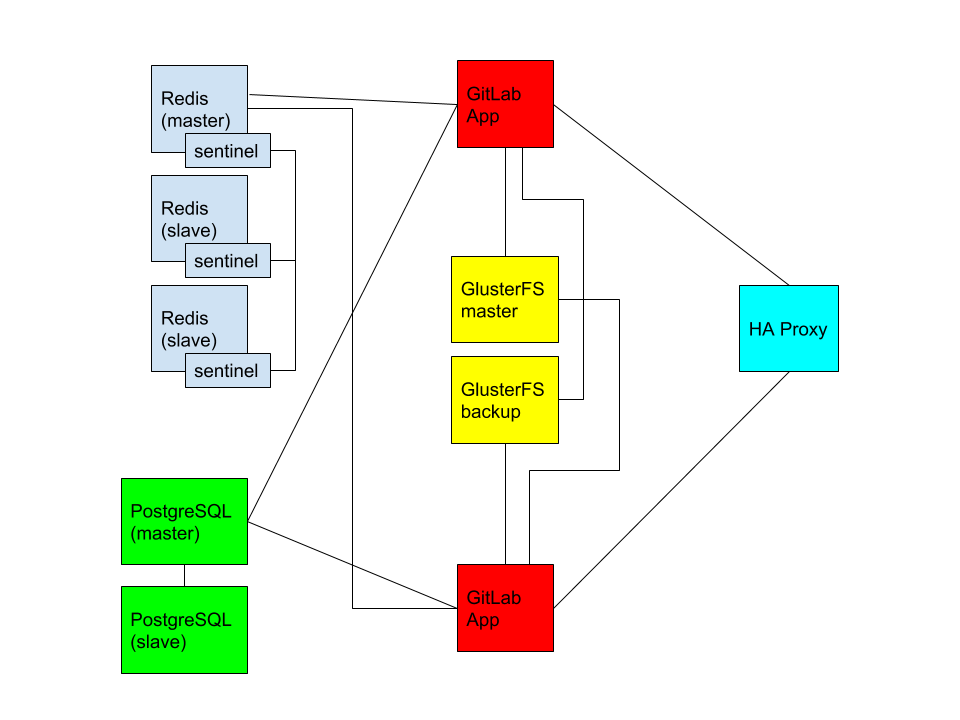
\includegraphics[width=15cm]{archBase.png}
    \caption{Arquitetura sem monitorização}
    \label{fig:archBase}
\end{figure}
Começando do nível mais baixo para o mais alto, o PostgreSQL é replicado usando duas das suas funcionalidades embutidas: Hot Standby~\cite{HotSt} e Streaming Replication~\cite{StRep}, de modo a garantir que os servidores estejam disponíveis e tenham leituras e escritas rápidas (desempenho). O Hot Standby permite que os servidores slave do PostgreSQL possam responder a queries de leitura, sendo as queries de escrita realizadas no servidor master. Já o Streaming Replication é a funcionalidade que mantém os dados continuamente coerentes entre os servidores PostgreSQL. Contudo, estas duas funcionalidades não garantem failover. Para isso, é necessário recorrer a outra ferramenta, por exemplo, repmgr, que garante que caso o servidor master vá abaixo seja escolhido um dos servidores slave para servir de master. Mesmo com a presença de failover e de Hot Standby esta arquitetura apresenta um ponto de falha no master, visto que grande parte dos pedidos vão continuar a passar pelo master. De modo a evitar tal situação devia ser usada uma arquitetura com vários masters (sincronizados ou sharding) e vários load balancers (com apenas um voltaríamos a ter o problema de um ponto de falha) que escalonassem os pedidos entre os masters.

Num nível acima, encontra-se o Redis. De modo a replicar o Redis recorreu-se a uma arquitetura master-slave, em que existe um servidor master que responde aos pedidos e em caso de falha, é escolhido um slave para servir de master (failover). O failover é garantido através do uso dos sentinels que estão em constante comunicação para saberem quando o master falha, para posteriormente escolherem um novo master e, caso o master anterior recupere, se torne um slave. Esta replicação garante a resiliência do Redis.

Devido há presença de mais do que um GitLab Application na arquitetura, há a necessidade de partilhar certos dados entre os mesmos e, por isso, há a necessidade de um sistema de ficheiros distribuído. É importante por isso, garantir a resiliência para que as aplicações não falhem por causa da falha do sistema distribuído. De modo a permitir uma mais fácil escalabilidade, foi escolhido o GlusterFS ao invés do NFS que é mais usualmente usado em conjunto com o GitLab. Ao usar o GlusterFS pode-se usar vários tipos de volumes de dados, sendo que o usado no nosso caso é um volume replicado. Esta replicação implica que todos os servidores a correr o GlusterFS que servem esse volume tem todos os mesmos dados e como tal, caso um falhe, pode ser substituído facilmente por outro. Esta troca não implica failover visto que, a aplicação que precisa dos dados, ao montar, indica um servidor principal e um ou mais de backup para que no caso do principal falhar, aceda aos servidores de backup. Seria possível garantir um melhor desempenho e um melhor equilíbrio caso o tipo de volume usado fosse distribuído com replicação (mantendo a resiliência dos dados), no qual, os dados estão distribuídos por vários volumes e em cada volume os dados são replicados por vários servidores~\cite{archGluster}. 

Já com os componentes PostgreSQL, Redis e GlusterFS construídos, é possível então construir os servidores com o GitLab Application. Foi usado o GitLab Community Edition, desativando os componentes PostgreSQL e Redis embutidos. Visto este ser o componente principal e como possui ainda vários serviços, como visto anteriormente na secção \ref{Arq}, há a necessidade de replicar este componente de modo a aumentar a escalabilidade bem como a resiliência caso um deles falhe. De modo a possibilitar tal escalabilidade é necessário usar load balancers de modo a distribuírem os pedidos recebidos pelos utilizadores, permitindo também o acesso por um único endereço IP. Esta abordagem apresenta problemas caso apenas seja usado um load balancer (o caso presente na arquitetura desenvolvida, visto que o GCP não possui floating IP's sendo por tal necessário usar por exemplo balanceadores internos do GCP~\cite{floatIP}) visto que, constitui um ponto de falha da arquitetura. Esta falha acontece caso o load balancer vá abaixo, fazendo com que toda a aplicação deixe de ser fornecida aos utilizadores, sendo por isso recomendável usar vários load balancers usando uma abordagem master-slave em que o failover é garantido usando por exemplo o Keepalived~\cite{keepalivedConf,keepalivedNg}.

Por fim, a impossibilidade de usar o protocolo HTTPS (mais seguro em termos de troca de mensagens entre arquitetura e utlizador) em vez do protocolo HTTP, deve-se há necessidade de comprar um domínio de modo a poder usar um certificado SSL/TLS gratuito da autoridade \href{https://letsencrypt.org/}{Let's Encrypt}, visto que, o Let's Encrypt não permite associar certificados a endereços IP. Para se usar um certificado associado ao endereço IP teria-se de recorrer a uma autoridade de certificados que possui tal funcionalidade sendo esses certificados pagos.

\subsection{Características do Ansible usadas}
Por forma, a desenvolver a arquitetura anteriormente descrita, o Ansible possui várias funcionalidades que permitem instalá-la e configurá-la no GCP de forma automática, sendo apenas necessário correr o comando e introduzir a palavra-passe quando o mesmo recorrer ao password store ao criar/ler as palavras-passes associadas aos componentes da arquitetura.
Foi usada uma estrutura de ficheiros do Ansible bastante usada que consiste no uso de roles, em que existe um ficheiro inicial que ``chama'' os vários roles consoante a tag presente nos hosts. É possível definir variáveis de input para cada role neste ficheiro. 

Exemplo de uma organização de ficheiros que respeita a estrutura do Ansible de modo a usar roles:
\begin{verbatim}
mainFolder
    playbook.yml
    roles
        role1
            tasks
                main.yml
            templates
                file1.j2
                file2.j2
        role2
            tasks
                main.yml
\end{verbatim}
O playbook.yml é o ficheiro inicial, sendo os roles todos definidos dentro da pasta roles. Cada role possui tasks e por vezes templates. Na pasta tasks existe um ficheiro main.yml que irá possuir as várias tasks a executar para um host ao qual lhe foi associado este role no ficheiro playbook.yml. Na pasta templates é comum existir ficheiros de configuração que são copiados para o host através do módulo template. Por exemplo, no role1, no main.yml existir uma task com o módulo template que copie o file1.j2 para /path/file1 no host. Nestes ficheiros de configuração é possível usar Jinja2, outra ferrramenta que veremos mais à frente.

De forma a criar as máquinas virtuais no GCP, o Ansible possui os módulos gcp\_compute\_disk, gcp\_compute\_network, gcp\_compute\_firewall, gcp\_compute\_address e gcp\_compute\_instance que permitem respetivamente a criação de discos, de redes, de firewalls, de endereços e de instâncias no GCP. É importante referir que para o uso destes módulos é preciso ter credenciais do GCP associadas aos módulos, sendo o caminho do ficheiro com as credenciais indicado nos playbooks na variável gcp\_cred\_file.

Para além destes módulos existem muitos mais, que permitem desde criar pastas e ficheiros (módulo file), substituir linhas num ficheiro segundo uma expressão regular (módulo lineinfile ou replace), correr um comando (módulo shell ou command), instalar packages (módulo apt no caso do SO Ubuntu), gerir serviços (reiniciar, começar, parar, etc) (módulo service ou systemd), cópia de ficheiros (módulo template), etc.

Cada módulo é personalizável, visto possuir campos a preencher que podem ser obrigatórios ou opcionais, permitindo assim executar uma task com um módulo da forma que é mais conveniente.
Uma funcionalidade do Ansible muito usada são as variáveis, que permitem guardar/ler valores necessários para a configuração/instalação da arquitetura. Em conjunto com o Jinja2 estas variáveis são bastante poderosas até porque o Jinja2 permite construit loops, if's, obter valores de variáveis, inserir conteúdo nos ficheiros de configuração como anteriormente referido, etc. Por forma a guardar valores existe 3 hipóteses: usar a macro vars e definir as variáveis dentro, usar a macro register ou usar o módulo set\_facts.
Por fim, outra funcionalidade muito usada é o uso de loop, with\_items, with\_nested associado a uma task. Isto permite que a task seja executada para cada item da lista indicada na secção do loop/with\_items. Já o with\_nested é bastante parecido só que um pouco mais complexo, visto serem loops aninhados.

\subsection{Estrutura Ansible usada no deployment}
Portanto, usando todas estas caracteristicas do Ansible foi usada a seguinte estrutura:
\begin{itemize}
    \item playbookProd.yml : chama pela ordem correta os respetivos roles, caso os roles sejam usados por ordem diferente pode originar erros, desde a aplicação não correr(crashar) até a própria instalação e configuração originar erro; é indicado aqui quantas instâncias são pretendidas e de que tipo (tag); as tags usadas são as mesmas que os nomes dos roles, ou seja, existe as seguintes tags: postgre-master, postgre-slave, redis-master, redis-slave, first-gfs, gfs, first-gitlab, gitlab, haproxy, elastic-kibana e logstash. Esta é a versão de produção.
    \item playbookTest.yml : o mesmo que o ficheiro anterior, mas sendo esta a versão de teste tem um outro role adicional jmeter, que instala o Apache JMeter de forma a correr testes
    \item run.sh : serve para correr a versão pretendida (Produção ou de Testes) 
    \item roles
        \begin{itemize}
            \item \textbf{gcp:} cria máquinas virtuais no GCP, sendo que as máquinas geradas dependem do input colocado no playbookProd.yml/playbookTest.yml consoante a versão escolhida; cada máquina tem a si associado um disco e um endereço que também são criados neste role; todas as instâncias estão na mesma rede que tem a si (rede) associada a firewall; primeiro role a ser executado
            \item \textbf{users:} cria o utilizador deployer, dá permissões sudo ao mesmo e adiciona chaves para possibilitar o acesso por ssh; aplicado a todas as instâncias
        	\item \textbf{postgre-master:} instala o PostgreSQL no servidor; cria a base de dados a ser usada pelo gitlab; cria o utilizador necessário para o GitLab(dono da base de dados criada); adiciona uma extensão (pg\_trgm) à base de dados criada (extensão necessária por causa do GitLab); apenas uma instância
        	\item \textbf{postgre-slave:} instala o PostgreSQL; associa-se ao servidor postgre-master e realiza a migração (cópia) da base de dados para si, de modo a poder responder a queries; uma ou mais instâncias que se acharem necessárias
        	\item \textbf{redis-master:} instala e configura o Redis de modo a servir de master que possui algumas diferenças de configuração em relação aos slaves; apenas uma instância
        	\item \textbf{redis-slave:} instala e configura servidores Redis a servirem de slave que se associam ao servidor Redis master; uma ou mais instâncias que se acharem necessárias
        	\item \textbf{first-gfs:} instala e configura o servidor com GlusterFS sendo que este cria o volume; apenas uma instância
        	\item \textbf{gfs:} restantes servidores GlusterFS que vão ter o volume criado em first-gfs; tem de ser executado antes do role first-gfs; uma ou mais instâncias que se acharem necessárias
        	\item \textbf{first-gitlab:} instala e configura o GitLab-CE, efetuando o seed da base de dados que deve ser apenas efetuado uma vez, bem como a geração de keys a serem usadas pelos restantes servidores aplicacionais; define a password do Admin(root) que pode ser posteriormente mudada; apenas uma instância
        	\item \textbf{gitlab:} instala e configura o GitLab-CE, são copiados para este as keys geradas pelo first-gitlab e não é efetuado o seed da base de dados; uma ou mais instâncias que se acharem necessárias
        	\item \textbf{haproxy:} instala e configura um load balancer HAProxy de modo a balancear os pedidos recebidos pelos servidores com GitLab Application(first-gitlab e gitlab); apenas uma instância
        	\item \textbf{elastic-kibana:} recebe os dados, interpreta-os (Elasticsearch) e mostra-os via web (Kibana); apenas uma instância
        	\item \textbf{logstash:} nodo que agrega e filtra todos os dados gerados pelos beats, passa os dados filtrados para o Elasticsearch; apenas uma instância
        	\item \textbf{beats:} instala e configura os beats usados para monitorização; aplicado a todas instâncias exceto aquelas com a tag elastic-kibana e logstash
        	\item \textbf{jmeter:} instala o Apache JMeter; corre testes; executado no host com tag igual a elastic-kibana
        \end{itemize}
\end{itemize}

Os roles elastic-kibana, logstash, beats e jmeter serão a seguir explicados a razão pela qual fazem parte do deployment mas, de forma abreviada os roles elastic-kibana, logstash e beats permitem instalar e configurar as ferramentas necessárias para monitorizar o sistema e o role jmeter permitirá correr testes na arquitetura.

Por fim, por forma a aceder a arquitetura deve ser acedido o endereço: \url{http://{{IPdoHAProxy}}/}.

\section{Monitorização} \label{Mon}
%TODO: Quais as ferramentas de monitorização utilizadas, as métricas escolhidas e a necessidade das mesmas.

De modo a monitorizar o sistema foi usada a ELK Stack usando a seguinte arquitetura:

\begin{figure}[H]
    \centering
    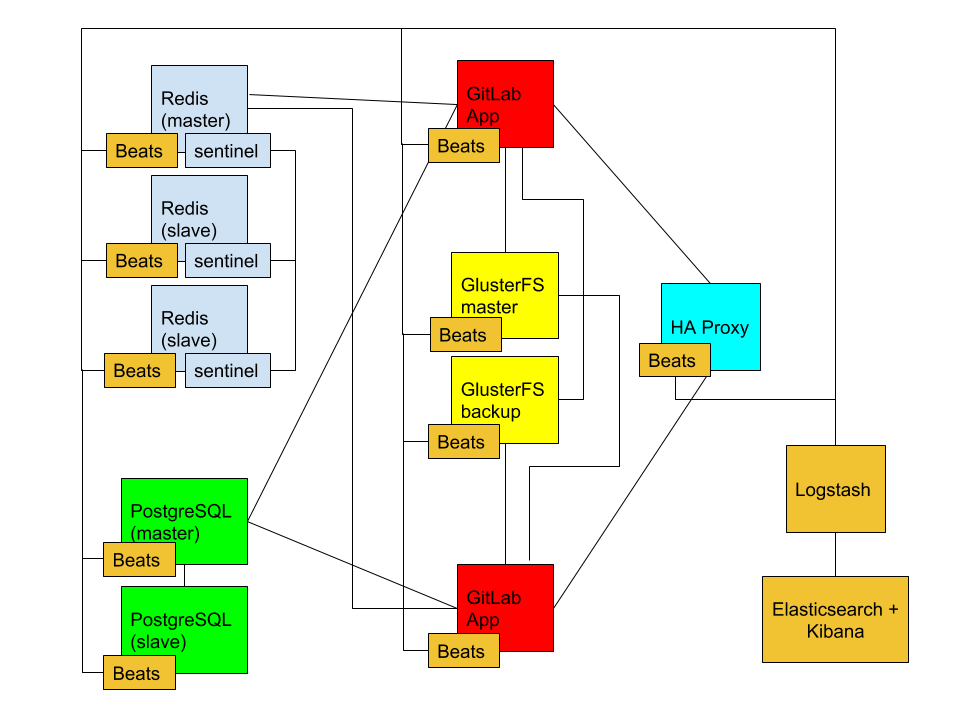
\includegraphics[width=15cm]{archMon.png}
    \caption{Arquitetura com monitorização}
    \label{fig:archBase}
\end{figure}
A ELK Stack consiste no uso de Elasticsearch, Logstash e Kibana, e são instalados beats nas máquinas a monitorizar, em que estes beats enviam os dados recolhidos para o Logstash. O Logstash filtra/trata os dados recebidos e envia-os para o Elasticsearch que organiza os dados de forma a serem visualizados no Kibana. Visto que, os componentes são independentes entre si, podem estar em diferentes máquinas. Na nossa arquitetura, como o Kibana é apenas um visualizador dos dados, ou seja, pouco esforço computacional, então o Kibana ficou junto com o Elasticsearch (pesado computacionalmente). Como o Logstash é também pesado computacionalmente decidiu-se colocar o Logstash numa máquina sozinho.

Por forma a perceber se cada componente precisa de mais RAM e CPU ou se é necessário replicar o componente, é importante monitorizar a RAM, o CPU e o I/O de todos os componentes. Pelas mesmas razões é importante perceber o desempenho de cada componente, ou seja, a latência e o débito. A latência é referente ao tempo que demora a responder a um pedido, e o débito é o número de pedidos que se consegue responder por unidade de tempo. De forma a monitorizar a RAM, o CPU e o I/O pode ser usado o Metricbeat, um dos beats da ELK Stack.

Estas métricas atrás referidas devem ser monitorizadas seja num ambiente de testes ou de produção. Contudo, num ambiente de produção é importante monitorizar também o número de pedidos recebidos por unidade de tempo. Esta métrica ajuda a perceber se os componentes instalados e configurados são mais (ou menos) do que o necessário e como tal o uso de recursos sem necessidade (ou falta de recursos), bem como o possível pagamento dos mesmos a cloud computing (como por exemplo o GCP) sem que as máquinas estejam a ser usadas, desperdiçando assim dinheiro e energia. Para isso, pode ser usado o Packetbeat, outro beat da ELK Stack. Para além de monitorizar a utilização (número de pedidos recebidos por unidade de tempo), é importante também monitorizar a eficiência (rácio entre débito e utilização) de forma a perceber se os recursos usados garantem um bom débito, ou se é necessário aumentar ou melhorar o hardware usado. Estas duas métricas utilização e eficiência, são recomendadas apenas para produção visto que, só no caso real é possível saber o número médio de utilizadores da arquitetura. Estas métricas também permitem saber se está no momento a acontecer algum pico de uso da arquitetura, permitindo assim, atuar de forma a não deixar o sistema ir abaixo devido a um grande fluxo de utilização.

Uma outra métrica a monitorizar é o espaço de disco, de forma a que caso algum dos componentes comece a ficar com pouco espaço de armazenamento, seja fornecido ao mesmo mais espaço de disco.

Já o uso do beat Filebeat, permite a partir do Kibana ver os log's das várias máquinas.

Em conclusão e pelas razões anteriormente referidas, os beats instalados em cada servidor, exceto o servidor com logstash e o servidor com elasticsearch+kibana, são o Metricbeat e o Filebeat. O Packebeat acabou por não ser instalado devido à interferência do mesmo com o GitLab originando erros inesperados. O Kibana pode ser consultado no endereço: \url{http://{{IPdoKibana}}:5601}.

\section{Avaliação} \label{Av}

O processo final na configuração de um sistema e antes de colocar o mesmo num ambiente de produção consiste em realizar uma avaliação da arquitetura implementada. 
avaliação é realizada por forma a identificar se é necessário aumentar a redundância de algum componente, ou se algum componente deve ser distribuído por máquinas diferentes bem como identificar, de forma antecipada, possíveis pontos de falha.

Com este intuito é usada uma ferramenta que permite criar e executar testes, ou seja, simular workloads referentes ao uso da aplicação, como se de utilizadores reais se trata-se. Esta ferramenta é o Apache JMeter. Por forma a gravar os passos feitos por um utilizador pode ser usada uma extensão do Chrome (BlazeMeter)~\cite{blazeM}, permitindo, através do JMeter, fazer com que uma grande quantidade de utilizadores façam os mesmos passos.


De forma a executar os seguintes testes é necessário antes criar um utilizador (ou usar o root).

Testes a realizar:~\cite{stressT,stressTest}
\begin{itemize}
    \item \textbf{Página inicial pelo HAProxy (lHAProxy.jmx):} executar um Stress Test que pretende detetar aproximadamente a quantidade de pessoas que podem estar a aceder a página inicial numa pequena quantidade de tempo. Este teste colocará à prova não só o HA Proxy, bem como os GitLab Applications's;
    \item \textbf{Página inicial por um dos GitLab Application (lGitLabApp.jmx):} o mesmo que o anterior teste, contudo apenas põe à prova um dos GitLab Application; simulando o funcionamento do sistema sem a atuação do HAProxy nem a existência de mais do que um GitLab Application.
\end{itemize}

Estes testes consistem em efetuar apenas um pedido GET, por utilizador, ao endereço IP da página inicial.

\subsection{Resultados da avaliação experimental}

De forma a correr os testes foram criados, para cada teste, um ficheiro inicial com a extensão .jmx com 10 iterações (aumenta o número de samples para a obtenção da latência e do througput), N threads (utilizadores) e um ramp time de 100 segundos, o que significa que a cada 100/N segundos uma thread(utilizador) começa a executar. Estes ficheiros .jmx foram criados com o JMeter mas podia ter sido usado o BlazeMeter addon para os criar, como anteriormente referido, de modo a definir os passos a serem realizados por cada utilizador e posteriormente, editar os ficheiros de forma a ter as características anteriormente referidas. De modo a gravar os passos realizados também pode ser usado o JMeter.

O JMeter foi instalado na mesma máquina que o Elasticsearch e Kibana, sendo que os ficheiros .jmx já criados são copiados pelo Ansible na fase de deployment. Posteriormente é possível copiar algum ficheiro por ssh com o comando scp (\verb|scp file IPJMeter:~/|).

De seguida ligamo-nos por ssh à maquina com o JMeter e realizam-se os passos seguintes.
Executam-se os testes usando a versão CLI(Command-Line Interface) do JMeter produzindo, no fim da execução de cada teste, um ficheiro .csv com os resultados (\verb|./jmeter -n -t test.jmx -l results.csv|). De seguida, usando a extensão do JMeter dashboard generator (\verb|./jmeter -g results.csv -o pastaDestino|)~\cite{genDash}, são geradas, a partir dos resultados, páginas HTML com gráficos de interpretação dos resultados, de forma a ser possível analisar mais facilmente os resultados. Os dois passos anteriores podem ser realizados com apenas um comando: \verb|jmeter -n -t test.jmx -l results.csv -e -o pastaDestino|.
Por fim estas páginas podem ser copiadas por scp para o nosso PC para serem posteriormente visualizadas no browser, sendo esta a forma como procedemos. Uma outra forma, sem cópia, seria permitir o acesso aos ficheiros do servidor pelo browser.

Por forma a descobrir o número máximo de utilizadores é escolhido um valor inicial N (neste caso N=100) e executa-se o teste. Caso haja erros reduz-se a quantidade de utilizadores, até chegar ao caso limite (em que não há erros). Caso não haja erros, aumenta-se o número de utilizadores para o dobro e repete-se: se houver erros reduz-se, senão aumenta-se de novo.

Antes da apresentação dos resultados é importante indicar que hardware foi usado em cada componente:
\begin{itemize}
    \item n1-standard-1 (1 vCPU(core lógico) e 3.75 GB de RAM): postgre-master, postgre-slave, redis-master, first-gfs, gfs, first-gitlab, gitlab, haproxy, logstash e elastic-kibana
    \item g1-small (0.5 vCPU(core lógico e 1.7 GB de RAM): redis-slave
\end{itemize}
É também importante referir que entre consecutivos testes do mesmo tipo apenas é alterado o número de threads (N), ou seja, tanto o ramp time (100 s) como número de loops (10) são mantidos constantes.

Resultados:
\begin{center}
  \begin{tabular}{| c | c | c | c | c |}
    \hline
    Tipo de Teste & Nº de Utilizadores & Percentagem de Erros & Latência média & Throughput \\ \hline
    lHAProxy.jmx & 55 & 0\% & 55.39 ms & 5.58 hits/ms \\ \hline
    lHAProxy.jmx & 550 & 1.85\% & 4544.54 ms & 38.84 hits/ms \\ \hline
    lGitLabApp.jmx & 55 & 0\% & 53.13 ms & 5.58 hits/ms \\ \hline
    lGitLabApp.jmx & 1000 & 0.17\% & 29597.16 ms & 24.03 hits/ms \\ \hline
  \end{tabular}
\end{center}

Os dois casos com 0\% de erro são bastante semelhantes porque o HAProxy só envia o pedido para o outro GitLab Application quando o primeiro começa a ficar sobrecarregado. A razão de a latência média ser maior com HAProxy deve-se ao tempo de comunicação adicional que existe entre HAProxy e GitLab Application enquanto que no caso sem HAProxy essa comunicação não existe.

Apesar de o teste lGitLabApp.jmx conseguir responder a 1000 utilizadores com uma percentagem de erro de 0.17\%, a sua latência média é muito alta (29597.16 ms $\approx$ 29.6 s). Isto acontece visto que como não existe tempo limite de resposta ou este é superior a 30 s no GitLab Application, os pedidos ficam à espera até obterem uma resposta, sendo essa resposta demorada devida à grande quantidade de pedidos. Ao invés disso, no caso com HAProxy, como existe um timeout menor (aumenta a percentagem de erros), este consegue apenas responder a 550 utilizadores com uma percentagem de erro de 1.85\% mas a latência média é menor, sendo apenas 4544.54 ms ($\approx$ 4.5 s).

Isto é verificável com o seguinte histograma:

\begin{figure}[H]
    \centering
    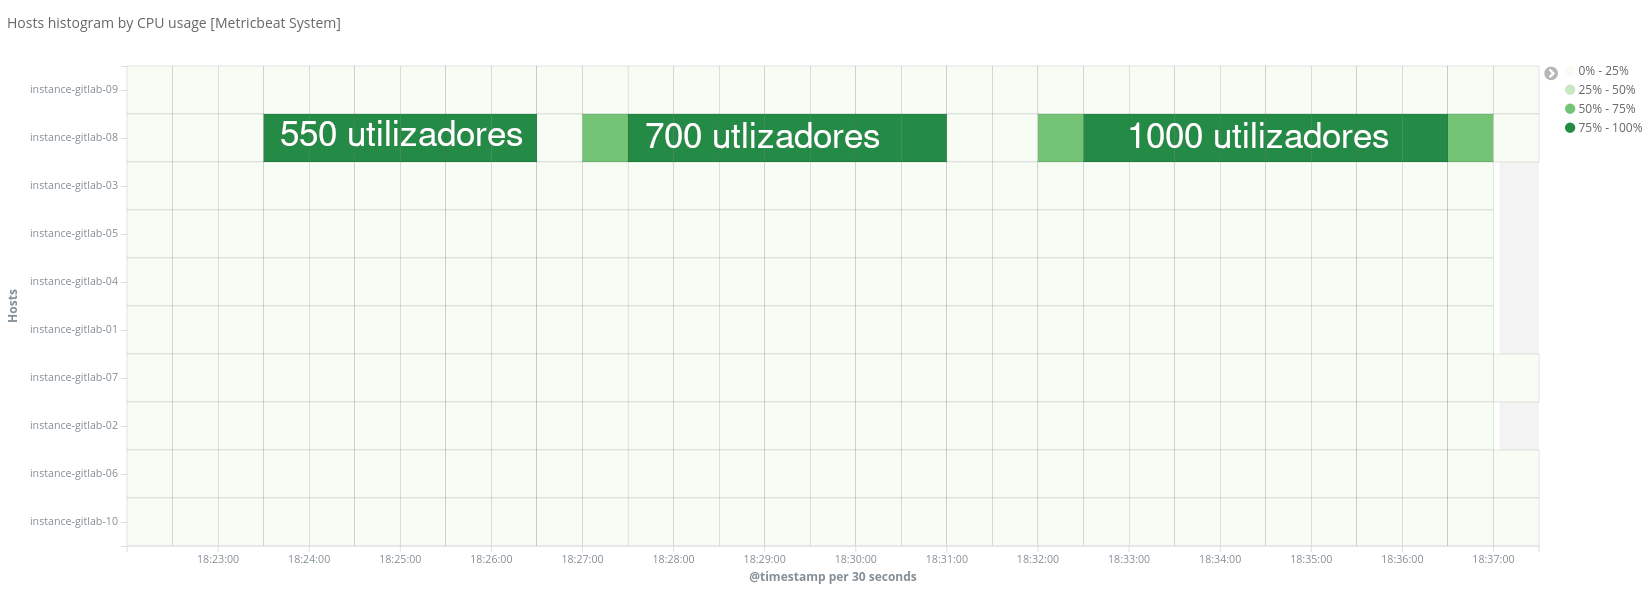
\includegraphics[width=15cm]{histAv.png}
    \caption{Histograma de uso do CPU com o aumento de utilizadores em cada teste}
\end{figure}

Quanto maior o número de utilizadores, maior é o tempo que o GitLab Application demora a responder a todos os utilizadores e como tal maior a latência média.

Ainda em relação ao primeiro tipo de teste (lHAProxy.jmx), aliando os testes realizados à monitorização da arquitetura é possível perceber que o grande peso deste teste situa-se nas GitLab Application's (instance-gitlab-08 e instance-gitlab-09) como é possível constatar pelos gráficos:

\begin{figure}[H]
    \centering
    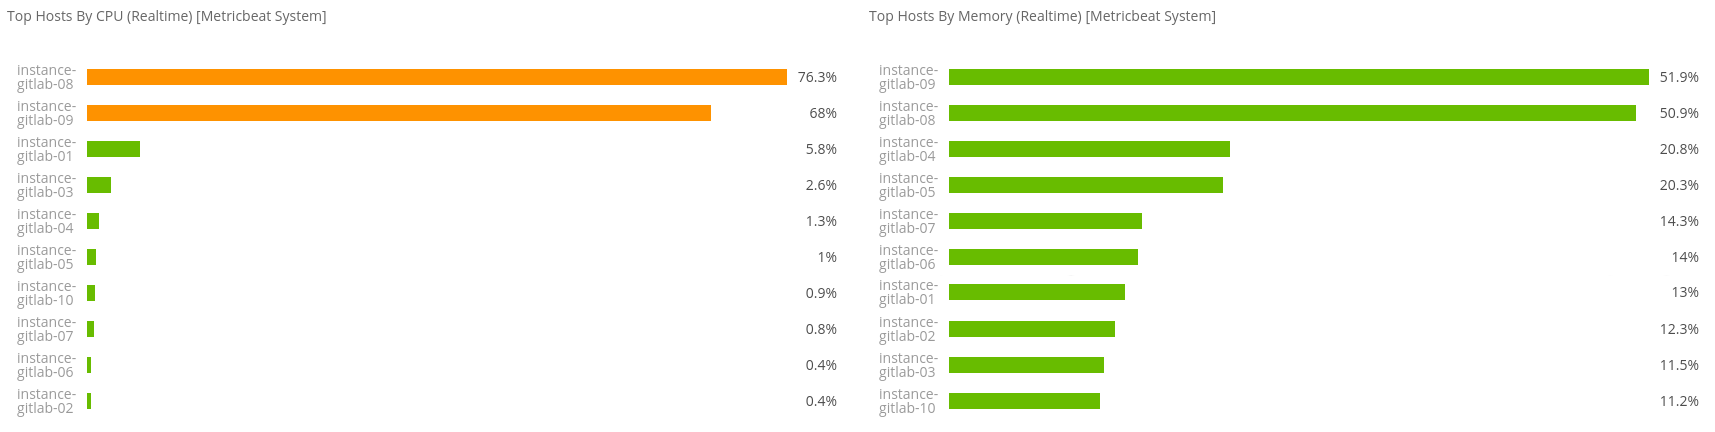
\includegraphics[width=15cm]{cpuMem.png}
    \caption{Percentagem de uso do CPU e da RAM após a execução de um teste com 550 utlizadores, ramp time de 100 segundos e 10 loops}
\end{figure}

\begin{figure}[H]
    \centering
    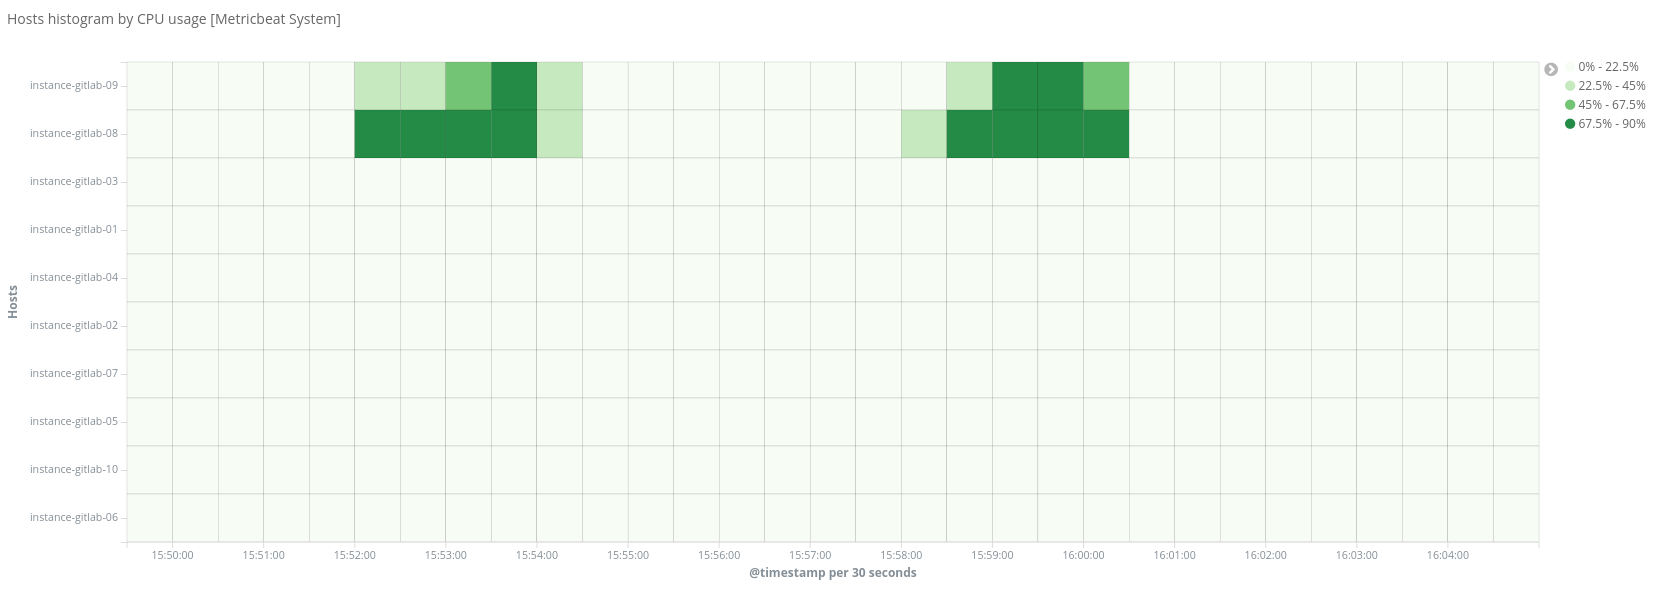
\includegraphics[width=15cm]{histCPU.png}
    \caption{Histograma de uso do CPU após a realização de vários testes}
\end{figure}

Com isto, pode concluir-se que, nas duas instâncias apresentadas, em vez de se usar uma configuração n1-standard-1, podia ser usada uma configuração de hardware um nível acima (n1-standard-2) visto neste caso, o hardware ser o bottleneck.

Os testes realizados permitem concluir que o número de utilizadores recomendado (\textbf{i.e.} que permite o normal funcionamento da aplicação) para o acesso à pagina inicial é de 55 utilizadores.

\subsection{Futura Avaliação}
Inicialmente o objetivo seria realizar os seguintes testes, sendo para os mesmos, é necessário criar um utilizador (ou usar o root) e criar um repositório:
\begin{itemize}
    \item \textbf{Login a toda a aplicação:} executar um Stress Test que pretende detetar aproximadamente a quantidade de pessoas que podem estar a realizar login numa pequena quantidade de tempo. Este teste colocará à prova não só o HA Proxy, bem como os GitLab Applications's, o Redis que armazena as sessões dos utilizadores e por fim, o PostgreSQL que armazena os dados dos utilizadores;
    \item \textbf{Login com acesso a um repositório a toda a aplicação:} para além do login, este teste envolve também o acesso à página de um projeto (repositório). Este segundo teste para além de pôr à prova os mesmos componentes que o anterior, põe também à prova o GlusterFS, visto os repositórios serem preferencialmente armazenados neste sistema de ficheiros distribuído. É também um Stress Test mas mais pesado que o anterior;
    \item \textbf{Login por um dos GitLab Application:} semelhante ao primeiro teste, contudo apenas põe à prova um dos GitLab Application, o Redis e o PostgreSQL;
    \item \textbf{Login com acesso a um repositório por um dos GitLab Application:} o mesmo que o segundo teste, coloca apenas à prova um dos GitLab Application, o Redis, o PostgreSQL e o GlusterFS.
\end{itemize}

A realização destes testes foi impossibilitada pela ocorrencia de um erro ao efetuar login através do JMeter que devolvia um erro com código 422 (Unprocessable Entity)~\cite{er422}, para o qual não foi encontrada uma causa (uma das origens deste erro poderia ser a existência de erros na introdução dos parâmetros, algo que não se verificou).

\newpage

\section{Conclusões} \label{Conc}

\par Com o trabalho desenvolvido é possível realizar instalações de produção e de teste, realizando pequenos ajustes (colocar/tirar um ou mais servidores replicados de um ou vários componentes) no ficheiro playbookProd.yml e playbookTest.yml, respetivamente, de acordo com o pretendido e, depois desses pequenos ajustes é apenas necessário correr a script run.sh com o parâmetro p (ex: \verb|./run.sh p|) para a instalação de produção e o parâmetro t (ex: \verb|./run.sh t|) para a instalação de teste.
\par Em relação à avaliação efetuada é possível concluir que para a arquitetura desenvolvida o número máximo recomendado para utilizadores (pelo menos no acesso à página inicial) é 55 utilizadores.
\par Por fim, apesar de um bom progresso realizado no trabalho, o mesmo carece ainda de muitas melhorias.
\par Em primeiro lugar, de forma a tornar a aplicação mais escalável e com melhor desempenho, falta a realização do failover do PostgreSQL bem como o uso de múltiplos masters, falta a replicação e failover do HAProxy e falta o uso de um volume distribuído replicado no GlusterFS.
\par Por outro lado, a instalação carece de segurança. Há a necessidade de restringir o acesso a várias portas a apenas alguns endereços IP. De forma a aumentar a segurança é também necessário habilitar o uso de HTTPS em vez de HTTP. 
\par Em relação à monitorização, o único ponto a melhorar seria a instalação do Packetbeat sem qualquer conflito com o GitLab. 
\par Já em relação à avaliação, era importante realizar mais testes, e testes que influenciassem toda a arquitetura (login com acesso a um repositório por exemplo), algo que não foi possível devido não se ter conseguido efetuar login via JMeter.

\newpage

\printbibliography

\end{document}
